\chapter{线性算子的谱理论}

谱理论关心的一些基本问题
\begin{enumerate}[itemindent=2em]
    \item $T_\lambda x=0$有非零解,即$\lambda$是$T$的特征值;
    \item $T_\lambda x=0$无非零解
\end{enumerate}

\section{谱集和正则点集}

\subsection*{\textsl{谱点和正则点}}

\begin{define}(\textbf{正则点})
    如果是$X$是复的\textsl{Banach}空间,$T$是从$\mathcal{L}(X)\subset X$到$X$的线性算子,$\lambda$称为\textbf{正则点}。
    如果$\lambda I- T$的值域$\mathcal{R}(\lambda I-T)$在$X$中稠密,并且$\lambda I-T$有连续逆算子,这样的$\lambda$全体称为$T$
    的正则点集,记为$\rho(T)$,有时把逆算子$(\lambda I-T)^{-1}$简记为$R_\lambda(T)$,称其为$T$的预解式。
\end{define}
\vspace*{1em}

\begin{define}(\textbf{谱集和谱点})
    正则点集$\rho(T)$的补集称为$T$的\textbf{谱集},记为$\sigma(T)$,即
    \begin{equation}
        \sigma(T)=\mathbb{C}/ \rho(T)
    \end{equation}

    如果$\lambda\in \sigma(T)$,则称$\lambda$为$T$的\textbf{谱点}。
\end{define}
\vspace*{1em}

\begin{define}(\textbf{点谱、连续谱和剩余谱})
    设$\sigma(T)$是线性算子$T$的谱集
    \begin{enumerate}[itemindent=2em]
        \item[$(1)$] 如果$\lambda I-T$不是一一对应的,$\lambda$称为$T$的\textbf{点谱},点谱全体记为$\sigma_p(T)$;
        \item[$(2)$] 如果$\lambda I-T$是一一对应的,且$\lambda I-T$的值域在$X$中稠密,但是它的逆算子是不连续的,$\lambda$称为$T$的\textbf{连续谱},连续谱全体记为$\sigma_c(T)$;
        \item[$(2)$] 如果$\lambda I-T$是一一对应的,但是$\lambda I-T$的值域在$X$中不稠密,则称$\lambda$为$T$的\textbf{剩余谱},剩余谱全体记为$\sigma_r(T)$;
    \end{enumerate}
\end{define}

\begin{figure}[H]
    \centering
    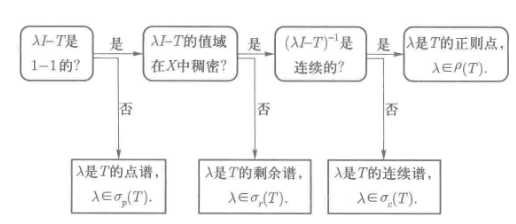
\includegraphics[scale=0.6]{figures/WX20240905-110243@2x.png}
    \caption{$T$的谱集}
\end{figure}

\begin{mdframed}
    \begin{theorem}
        设$H$是\textsl{Hilbert}空间,$T\in \mathcal{B}(H)$,则
        \begin{equation}
            \sigma(T^*)=\{\overline{\lambda}|\lambda\in \sigma(T)\}
        \end{equation}
    \end{theorem}
\end{mdframed}

\textbf{proof.}\hspace*{0.5em} 对$\lambda \in \rho(T)$,
\begin{equation}
    R_{\overline{\lambda}}(T^*)=(\overline{\lambda}I-T^*)^{-1}=[(\lambda I-T)^{-1}]^*=(R_\lambda(T))^T
\end{equation}

\subsection*{\textsl{特征值和特征元素}}

$T$的零空间$\mathcal{N}(\lambda I-T)$称为$T$关于$\lambda$的\textbf{特征子空间},它包括零元素和$T$的全体关于$\lambda$的特征元素,$T$关于$\lambda$的特征子空间的维数$\dim\mathcal{N}(\lambda I-T)$称为
特征值$\lambda$的\textbf{几何重数}。

\begin{example}
    设$H=L^2(-\infty,\infty)$,$T:H\rightarrow H$,$y=Tx$,其中
    \begin{equation}
        y(t)=\int_{\infty}^{t}e^{-(t-\tau)}d\tau
    \end{equation}

  当$\mathcal{D}(T)=H$,$\mathcal{R}(T)\subset H$,当$x(t)=e^{i\omega t}$时
    \begin{eqnarray}
        \int_{-\infty}^{t}e^{-(t-\tau)}e^{i\omega \tau}d\tau=\int_{-\infty}^{t}e^{-t}e^{(1+i\omega)\tau}d\tau=\frac{1}{1+i\omega}e^{i\omega t}
    \end{eqnarray}

    但这并不意味着$1/(1+i \omega)$是算子$T$的连续谱,事实上$x(t)= e^{i\omega t}\notin L^2(-\infty, \infty)$,可以证明$1/(1+i\omega)$是算子$T$的连续谱。
\end{example}

\begin{mdframed}
    \begin{proposition}
        设$\lambda_1,\lambda_2,\cdots,\lambda_n$是线性算子$T$的互不相关的特征值,$x_1,\cdots,x_n$是对应的特征元素,则$x_1,x_2,\cdots, x_n$是线性无关的。
    \end{proposition}
\end{mdframed}

\begin{mdframed}
    \begin{theorem}
        证明:$dim(\mathcal{N}(\lambda I- T))+dim(\mathcal{R}(\lambda I- T))=dim X$
    \end{theorem}
\end{mdframed}

\subsection*{\textsl{闭算子的正则点}}

\begin{mdframed}
    \begin{theorem}
        设$X$是\textsl{Banach}空间,$T$是从$\mathcal{D}(T)\subset X$到$X$的闭线性算子,那么对于所有的$\lambda\in \rho(T)$,
        $(\lambda I-T)^{-1}$是一个定义在全空间上的有界线性算子。
    \end{theorem}
\end{mdframed}

\section{有界线性算子的谱集}

\subsection*{\textsl{有界线性算子的谱集是有界集}}

\begin{mdframed}
    \begin{theorem}
        设$X$是\textsl{Banach空间},$T\in \mathcal{B}(X)$,如果$\Vert T\Vert<1$,则算子$I-T$有有界逆算子,并且
        \begin{equation}
            \begin{aligned}
                & (I-T)^{-1}=\sum^{\infty}_{n=0} T^n \\
                & \Vert (I-T)^{-1}\Vert\leqslant \frac{1}{1-\Vert T\Vert}
            \end{aligned}
        \end{equation}
    \end{theorem}
\end{mdframed}

\begin{mdframed}
    \begin{theorem}
        设$X$是\textsl{Banach空间},$T\in \mathcal{B}(X)$,则$\sigma(T)$是有界集
    \end{theorem}
\end{mdframed}

\subsection*{\textsl{有界线性算子的谱集是闭集}}

\begin{mdframed}
    \begin{theorem}
        设$T$是\textsl{Banach空间}$X$到$X$的线性算子,$\lambda\in \rho(T)$,且$|\mu|<\Vert (\lambda I-T)^{-1}\Vert^{-1}$,则$\lambda+\mu\in \rho(T)$,即$\rho(T)$是一个开集。
    \end{theorem}
\end{mdframed}

\subsection*{\textsl{有界线性算子谱集非空}}

\begin{mdframed}
    \begin{lemma}
        设$\lambda,\mu\in \rho(T)$,
        \begin{equation}
            R_\lambda(T)-R_\mu(T)=(\mu-\lambda)R_{\lambda}(T)R_\mu(T)
        \end{equation}
    \end{lemma}
\end{mdframed}

\begin{mdframed}
    \begin{theorem}
        在正则集$\rho(T)$中,预解式
        \begin{equation}
            R_\lambda(T):\lambda\in \rho(T)\subset \mathbb{C}\rightarrow \mathcal{B}(X)
        \end{equation}

        是关于$\lambda$的算子值解析函数。
    \end{theorem}
\end{mdframed}

\begin{mdframed}
    \begin{theorem}
        设$T$是有界线性算子,则$\sigma(T)\neq \emptyset$
    \end{theorem}
\end{mdframed}

\subsection*{\textsl{有界线性算子的谱半径}}

我们称$r_\sigma(T)=\inf\limits_k\Vert T^k\Vert^{\frac{1}{k}}=\lim\limits_{k\rightarrow \infty}\Vert T^k\Vert^{\frac{1}{k}}$为有界线性算子$T$的\textbf{谱半径}。

\begin{mdframed}
    \begin{theorem}
        设$T\in \mathcal{B}(X)$,则极限
        \begin{equation}
            r_\sigma(T)=\lim_{k\rightarrow\infty}\Vert T^k\Vert^{\frac{1}{k}}=\inf \Vert T^k\Vert^{\frac{1}{k}}
        \end{equation}

        存在
    \end{theorem}
\end{mdframed}

\begin{mdframed}
    \begin{theorem}
        $T\in \mathcal{B}(X)$,则$r_\sigma(T)=\sup\limits_{\lambda\in \sigma(T)}|\lambda|$
    \end{theorem}
\end{mdframed}

\section{有界子共轭线性算子的谱}

\section{紧线性算子的谱}